\chapter{算法设计}\label{chap:method}\label{chap:algorithm}

本章说明从复杂区域输入到Pareto部署方案输出的完整计算流程。先用区域分解把不规则多边形变成若干可编码凸子区域，再用坐标变换把粒子的归一化坐标放回物理空间，最后由MOPSO-DT在第三章定义的目标函数上迭代搜索。图~\ref{fig:workflow_overview}给出了这一流程的整体关系。

\begin{figure}[!htbp]
\centering

\includegraphics[width=0.88\linewidth]{figures/coordinate_transform_pipeline.pdf}
\caption{区域分解、坐标变换与部署优化流程。}
\label{fig:workflow_overview}
\end{figure}

图~\ref{fig:architecture}把实现拆成三层。输入层读取部署区域、雷达参数和任务点；预处理层生成凸子区域、区域编码和坐标映射；优化层只接收可评估的部署方案，并维护外部Pareto档案。这样的划分使NSGA-II、MOEA/D和SPEA2等基线也能复用同一套评估函数。

\begin{figure}[!htbp]
\centering
\includegraphics[width=0.86\linewidth]{figures/fig_architecture.pdf}
\caption{MOPSO-DT系统架构。}
\label{fig:architecture}
\end{figure}

\section{区域分解算法}

复杂区域不能直接交给标准PSO更新，否则粒子经常落在禁入区域或多边形外部。本文先使用Hertel-Mehlhorn思路将$\mathcal{R}$分解为$K$个凸多边形$\mathcal{P}=\{P_1,P_2,\ldots,P_K\}$。图~\ref{fig:decomposition_pipeline}以带空洞矩形为例展示中间过程：先识别连通分量，再用切割消除空洞，随后分解为凸子区域并分配二进制编码。优化器中的离散变量选择子区域，连续变量决定子区域内的位置。

\begin{figure}[!htbp]
\centering

\includegraphics[width=0.86\linewidth]{figures/decomposition_pipeline.pdf}
\caption{带空洞部署区域的凸分解流程示例。}
\label{fig:decomposition_pipeline}
\end{figure}

在图示流程基础上，算法~\ref{alg:decomposition}给出了区域凸分解的主要步骤。

\Needspace{0.36\textheight}
\begin{algorithm}
\caption{区域凸分解算法}
\label{alg:decomposition}
\begin{algorithmic}[1]
\STATE 输入：部署区域多边形$\mathcal{R}$（可含空洞）
\STATE 输出：凸多边形集合$\mathcal{P}$，二进制编码映射
\STATE 对$\mathcal{R}$进行连通分量分析，分解为$C$个独立区域
\FOR{$c = 1$ \TO $C$}
    \STATE 检测区域$c$中的空洞
    \IF{存在空洞}
        \STATE 使用双线段切割消除空洞~\cite{Chazelle1982}
    \ENDIF
    \STATE 对无空洞多边形进行约束三角剖分
    \STATE 贪心合并相邻三角形形成凸多边形
\ENDFOR
\STATE 为每个凸多边形$P_k$分配唯一的$N_{\text{bin}}$位二进制编码
\STATE 返回 $\mathcal{P}, N_{\text{bin}}$
\end{algorithmic}
\end{algorithm}

算法~\ref{alg:decomposition}输出的凸多边形并集与原区域一致，且每个子区域具有唯一二进制编码。其复杂度为$O(n\log n)$，其中$n$为多边形顶点数。本文后续只在这些编码区域内搜索，避免在原始非凸边界上反复做可行性修正。

为说明该分解策略并不局限于单一几何形状，图~\ref{fig:decomposition_variety}给出了多类典型区域的处理结果。对于L形、T形、十字形等凹多边形，算法通过切分凹角得到少量凸子区域；对于不连通区域或带多个空洞的区域，算法先分离连通分量或消除内部空洞，再统一分配区域编码。这一过程使后续优化器不需要直接处理复杂的几何约束。

\begin{figure}[!htbp]
\centering

\includegraphics[width=0.88\linewidth,height=0.44\textheight,keepaspectratio]{figures/decomposition_variety.pdf}
\caption{代表性区域形状的凸分解结果。}
\label{fig:decomposition_variety}
\end{figure}

\section{坐标变换}

完成区域分解后，还需要把$[0,1]^2$中的粒子坐标转换成对应凸多边形内的物理坐标。本文采用垂直交点法。

图~\ref{fig:coordinate_transform_overview}展示了这种映射的含义。粒子不会先落到外接矩形再被裁剪，而是根据目标凸多边形在当前横坐标处的有效上下边界重新定位。这样，速度更新仍在归一化空间中完成，但得到的物理位置保持可行，边界附近候选点也不必因越界而被简单丢弃。

\begin{figure}[!htbp]
\centering
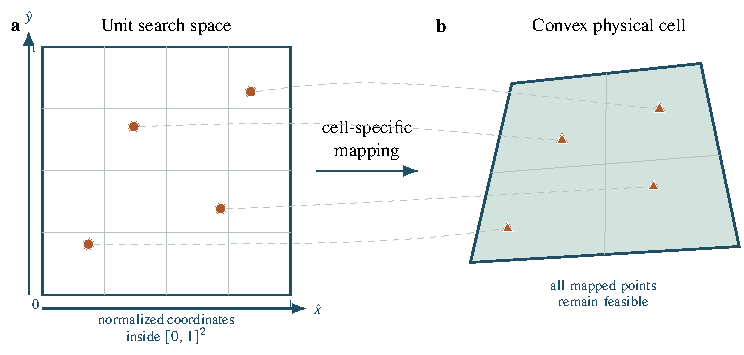
\includegraphics[width=0.88\linewidth]{figures/coordinate_transform_overview.pdf}
\caption{归一化搜索空间到凸多边形物理空间的映射。}
\label{fig:coordinate_transform_overview}
\end{figure}

算法\ref{alg:coordinate_transform}给出垂直交点坐标变换。算法先用目标凸多边形的轴对齐包围盒确定物理垂线，再计算垂线与多边形边界的交点，最后根据归一化纵坐标在有效线段内插值得到物理坐标。该步骤把约束处理前置到坐标映射中，减少后续优化循环中的非法点过滤。

\Needspace{0.34\textheight}
\begin{algorithm}
\caption{垂直交点坐标变换}
\label{alg:coordinate_transform}
\begin{algorithmic}[1]
\STATE 输入：凸多边形$P_k$，归一化坐标$(\hx, \hy) \in [0,1]^2$
\STATE 输出：物理坐标$(x, y) \in P_k$
\STATE 计算$P_k$的轴对齐包围盒：$[x_{\min}, x_{\max}] \times [y_{\min}, y_{\max}]$
\STATE 根据$\hx$确定垂直扫描线横坐标：$x = x_{\min} + \hx \cdot (x_{\max} - x_{\min})$
\STATE 构造垂直扫描线$L_x=\{(x,y)\mid y\in[y_{\min},y_{\max}]\}$
\STATE 逐边计算$L_x$与$P_k$边界的交点，得到交点集合$\mathcal{I}_x$
\STATE 合并由顶点重合或数值误差产生的重复交点
\STATE 按纵坐标对$\mathcal{I}_x$升序排序
\STATE 根据凸多边形内部线段确定当前$x$处的下边界$y_{\mathrm{low}}(x)$
\STATE 根据同一有效线段确定当前$x$处的上边界$y_{\mathrm{high}}(x)$
\STATE 若$y_{\mathrm{high}}(x)=y_{\mathrm{low}}(x)$，令$y=y_{\mathrm{low}}(x)$
\STATE 否则令$y = y_{\mathrm{low}}(x) + \hy \cdot (y_{\mathrm{high}}(x)-y_{\mathrm{low}}(x))$
\STATE 得到物理空间中的可行候选点$(x,y)$
\STATE 返回 $(x, y)$
\end{algorithmic}
\end{algorithm}

图~\ref{fig:coordinate_transform_detail}进一步给出了垂直交点法的三个典型计算位置。给定$\hat{x}$后，算法先确定物理空间中的垂直扫描线，再计算该扫描线与凸多边形边界的下交点$l_y(x)$和上交点$u_y(x)$，最后按$\hat{y}$在该有效线段内插值得到物理坐标。该步骤使不同形状的凸子区域均可使用同一套连续变量更新公式。

\begin{figure}[!htbp]
\centering

\includegraphics[width=0.88\linewidth]{figures/coordinate_transform_detail.pdf}
\caption{垂直交点坐标变换步骤。}
\label{fig:coordinate_transform_detail}
\end{figure}

坐标变换的作用可以概括为两点：一是保证粒子更新后的物理位置仍在合法区域内，二是减少外接矩形采样造成的边界候选点损失。该变换并不声称在面积意义上严格均匀；在本文中，它主要承担约束处理和边界可达性的功能。

\section{MOPSO-DT多目标优化算法}

\subsection{粒子编码}

每个粒子代表一种完整的雷达部署方案。对于$J$个雷达和$N_{\text{bin}}$位二进制区域编码，粒子的位置向量为：
\begin{equation}
\mathbf{\Phi} = [\hx_1, \hy_1, b_1^1, \ldots, b_1^{N_{\text{bin}}}, \hx_2, \hy_2, b_2^1, \ldots, b_J^{N_{\text{bin}}}]
\label{eq:particle_encoding}
\end{equation}
\noindent{}其中$(\hx_j, \hy_j) \in [0,1]^2$为第$j$个雷达的归一化坐标（连续变量），$b_j^1, \ldots, b_j^{N_{\text{bin}}} \in \{0,1\}$为区域索引的二进制编码（离散变量）。该编码同时优化连续坐标和离散区域选择，属于混合变量优化问题。

\subsection{更新规则}

连续变量更新采用标准PSO速度-位置更新：
\vspace{-0.5\baselineskip}
\begin{align}
v_i^d(t+1) ={}& w(t) \cdot v_i^d(t)
 + c_1 \cdot r_1 \cdot \left(p_i^{d,\text{best}} - x_i^d(t)\right) \notag\\
& + c_2 \cdot r_2 \cdot \left(g^{d,\text{best}} - x_i^d(t)\right)
\label{eq:continuous_update}
\end{align}
\vspace{-1.7\baselineskip}

二进制变量更新通过交叉和变异操作完成：
\vspace{-0.5\baselineskip}
\refstepcounter{equation}\label{eq:binary_crossover}
\begin{equation*}
\tilde{b}_j^k(t+1) =
\begin{cases}
b_{p,j}^{k,\text{best}}, & r_1 < p_c,\ r_2 < \frac{c_1}{c_1+c_2}, \\
b_{g,j}^{k,\text{best}}, & r_1 < p_c,\ r_2 \geq \frac{c_1}{c_1+c_2}, \\
b_j^k(t), & r_1 \geq p_c,
\end{cases}
\tag*{\raisebox{-1.6\baselineskip}{(\theequation)}}
\end{equation*}
\vspace{-0.25\baselineskip}
\noindent{}其中$b_{p,j}^{k,\text{best}}$和$b_{g,j}^{k,\text{best}}$分别表示个体最优和全局领导者中的区域选择编码，$p_c$为交叉概率。随后执行独立变异：
\refstepcounter{equation}\label{eq:binary_mutation}
\begin{equation*}
b_j^k(t+1) =
\begin{cases}
1-\tilde{b}_j^k(t+1), & r_3 < p_m, \\
\tilde{b}_j^k(t+1), & r_3 \geq p_m,
\end{cases}
\tag*{\raisebox{-0.8\baselineskip}{(\theequation)}}
\end{equation*}
\vspace{-1.0\baselineskip}

\subsection{动态参数策略}

惯性权重$w(t)$采用standard线性递减策略$w(t)=0.9-0.5\cdot t/T_{\max}$。该设置在前期保留较大的速度延续能力，便于跨子区域探索；迭代后期$w(t)$降低，粒子更容易围绕已发现的非支配区域细化搜索~\cite{Shi1998}。

变异概率$p_m(t)$采用动态下界策略$p_m(t)=\max(p_m^{\text{base}}, w(t)/N_P)$，其中$p_m^{\text{base}}=0.01$，$N_P$为粒子数。这样做是为了避免迭代后期区域编码完全停止扰动，尤其是在不连通区域或带空洞区域中保留少量跨区域尝试。

\subsection{全局最优选择}

在多目标场景中，"全局最优"不再唯一。本文比较以下两种选择策略：

\begin{itemize}
    \item 随机选择（random）：从外部档案中均匀随机选择一个非支配解作为全局最优。简单高效，但可能加剧解的聚集，使得粒子更倾向于飞向Pareto前沿上已经密集的区域~\cite{Coello2004}。
    \item 拥挤度加权轮盘赌（crowding）：按照拥挤距离加权概率，从外部档案中选择全局最优。拥挤距离越大的解被选中的概率越高，鼓励粒子向Pareto前沿的稀疏区域移动，从而自动填补前沿缺口、提升解的分布均匀性~\cite{Raquel2005}。
\end{itemize}

本文采用拥挤加权策略，主要是因为部署问题只有ECR和$J_{\min}$两个目标，前沿稀疏区域具有明确的工程含义：这些区域对应覆盖和压制之间较少被探索的折中方案。随机选择领导者实现简单，但粒子可能反复靠近档案中的密集区域；拥挤加权选择则提高稀疏解被选中的概率，使搜索压力更多分配到前沿缺口处。该思路与NSGA-II中的拥挤距离机制以及MOPSO领导者选择方法一致~\cite{Deb2002,Raquel2005}。

近年的多目标粒子群改进方法提供了更复杂的领导者预测、指标融合或分解选择机制~\cite{Liu2023,Wang2024,Zhang2024,Xu2024,Sun2024,Ma2025}。本文没有引入这些额外结构，原因是当前场景为双目标部署问题，拥挤距离已经能提供足够直接的分布控制。第五章实验也显示，crowding策略相对random策略能在Spacing上取得35.7\%至54.0\%的改善。

\subsection{外部档案维护}

外部档案$\mathcal{A}$维护搜索过程中发现的非支配解，这是MOPSO处理多目标问题时保持历史非支配信息的常用机制~\cite{Coello2004,Mostaghim2003}。当新解加入时：
\begin{enumerate}
    \item 将新解与档案中所有解进行Pareto支配比较
    \item 若新解被档案中任一解支配，则丢弃新解
    \item 若新解支配档案中部分解，则删除被支配的旧解，并添加新解
    \item 若档案大小超过预设容量，删除拥挤距离最小的解
\end{enumerate}

\subsection{算法主循环}

算法\ref{alg:mopso_dt}汇总了MOPSO-DT部署优化流程。输入为部署区域、节点数量和优化参数；预处理阶段完成区域凸分解和粒子初始化；迭代阶段依次执行领导者选择、连续坐标更新、二进制编码更新、坐标映射、目标函数评估和档案维护。输出的$\mathcal{A}$是一组非支配部署方案，而不是单个固定解。

主循环中，连续变量给出节点在所选凸子区域内的归一化坐标，并经算法~\ref{alg:coordinate_transform}映射为物理位置；二进制变量决定节点所属凸子区域。两类变量共同保留PSO更新形式，同时在评估前完成可行域约束，避免节点落入非部署区域、空洞或不连通区域之外。

评估时，新部署方案在ECR和$J_{\min}$双目标空间中比较；个体最优保存粒子历史可行方向，外部档案保存群体非支配方案，并在超限时用拥挤距离保留稀疏前沿解。因此，最终输出仍是一组覆盖--压制折中候选方案。

\Needspace{0.48\textheight}
\begin{algorithm}
\caption{MOPSO-DT多目标部署优化}
\label{alg:mopso_dt}
\begin{algorithmic}[1]
\STATE 输入：区域$\mathcal{R}$，雷达数量$J$
\STATE \quad 参数$N_P, T_{\max}, c_1, c_2, w_{\text{strategy}}, p_m^{\text{base}}$
\STATE 输出：Pareto最优部署方案集合$\mathcal{A}$
\STATE 初始化：
\STATE \quad 运行区域分解算法（算法~\ref{alg:decomposition}）$\to \mathcal{P}, N_{\text{bin}}$
\STATE \quad 随机初始化$N_P$个粒子（均匀分布归一化坐标+二进制编码）
\STATE \quad 评估每个粒子，初始化外部档案$\mathcal{A}$为初始非支配解
\FOR{$t = 1$ \TO $T_{\max}$}
    \STATE 计算$w(t)$和$p_m(t)$
    \FOR{每个粒子$i$}
        \STATE 选择全局最优$\mathbf{g}^{\text{best}}$（random或crowding策略）
        \STATE 更新连续坐标：式(\ref{eq:continuous_update})
        \STATE 更新二进制编码：式(\ref{eq:binary_crossover})--(\ref{eq:binary_mutation})
        \STATE 坐标变换（算法~\ref{alg:coordinate_transform}）$\to$ 物理位置
        \STATE 评估目标函数$f_1, f_2$
\algstore{mopso_dt_break}
\end{algorithmic}
\end{algorithm}

\vskip 20pt
\noindent\makebox[\linewidth][r]{\zihao{-5}\songti 续算法~\ref{alg:mopso_dt}\hspace{2em}}\par
\hrule height.8pt depth0pt \kern2pt
\begin{algorithmic}[1]
\algrestore{mopso_dt_break}
        \STATE 更新个体最优$\mathbf{p}_i^{\text{best}}$（Pareto支配关系）
    \ENDFOR
    \STATE 更新外部档案$\mathcal{A}$（Pareto支配+拥挤距离截断）
\ENDFOR
\STATE 返回 $\mathcal{A}$
\end{algorithmic}
\kern2pt\hrule\relax
\vskip 20pt

从迭代执行角度看，MOPSO-DT的核心循环可概括为图~\ref{fig:mopso_iteration_pipeline}。粒子初始化后反复经历速度/位置更新、坐标变换、目标函数评估和Pareto档案更新；惯性权重$w(t)$和变异概率$p_m(t)$随迭代动态调整，使前期保持较强全局探索，后期逐步转向局部收敛与前沿补全。

\begin{figure}[!htbp]
\centering

\includegraphics[width=0.96\linewidth]{figures/fig_pipeline.pdf}
\caption{MOPSO-DT迭代流程。}
\label{fig:mopso_iteration_pipeline}
\end{figure}

\section{公平对比协议}

为避免不同算法之间由于编码、目标函数或评价预算不同而产生不公平比较，本文在第五章的多算法对比中采用统一协议。所有算法均使用与MOPSO-DT相同的混合变量编码：每个雷达节点包含两个归一化连续坐标和$N_{\text{bin}}$位区域编码；所有候选解均调用同一评估函数计算$f_1=1-\text{ECR}$和$f_2=J_{\text{ref}}/(J_{\min}+J_{\text{ref}})$；每个方法在同一场景、同一随机种子集合和同一评价预算$N_P T_{\max}$下运行。

对比算法包括原始MOPSO-DT配置（legacy惯性权重与random全局最优选择）、随机搜索、NSGA-II、MOEA/D和SPEA2。NSGA-II、MOEA/D和SPEA2分别代表非支配排序、分解和强度Pareto适应度三类经典多目标进化思想~\cite{Deb2002,Zhang2007,Zitzler2001}。NSGA-II和SPEA2采用与本文实现一致的连续变量交叉、二进制均匀交叉和位翻转变异；MOEA/D采用双目标权重向量分解和Tchebycheff标量化子问题。上述基线用于检验本文MOPSO-DT配置在相同部署模型中的相对表现，而非复现各文献算法的全部工程细节。

\section{算法复杂度分析}

MOPSO-DT算法的主要计算开销来自每轮迭代中的粒子评估。对于$M$个任务点、$J$个雷达、$N_P$个粒子和$T_{\max}$次迭代：

\begin{itemize}
    \item 每次粒子评估需要计算$M \times J$的探测概率矩阵和等效干扰强度矩阵，复杂度为$O(M \cdot J)$
    \item 每轮迭代需评估$N_P$个粒子，总复杂度为$O(N_P \cdot M \cdot J)$
    \item 外部档案维护的复杂度为$O(|\mathcal{A}| \log |\mathcal{A}|)$
    \item 总时间复杂度：$O(T_{\max} \cdot N_P \cdot M \cdot J + T_{\max} \cdot |\mathcal{A}| \log |\mathcal{A}|)$
    \item 空间复杂度：$O(N_P \cdot J \cdot (2 + N_{\text{bin}}) + |\mathcal{A}|)$
\end{itemize}

在实际应用中，通过Numba即时编译（Just-in-Time, JIT）和向量化矩阵运算，MOPSO-DT可实现显著的运行时加速。以$T_{\max}=500, N_P=50, M=100, J=8$的典型配置为例，整个优化过程在消费级中央处理器（Central Processing Unit, CPU，Intel Core i7-13700H）上耗时156.3秒（约2.6分钟）。

\FloatBarrier

\ctexset{paragraph/number={\AlphAlph{\value{paragraph}}}}

\paragraph{区域分解对搜索空间的作用}
区域分解的目的不是改变原始部署任务，而是将复杂区域中的连续搜索过程组织得更加明确。对于不规则任务区域，若直接在全局坐标系中搜索，粒子位置更新既要满足边界约束，又要兼顾覆盖质量和网络性能，搜索空间中会存在大量无效或低质量候选点。通过先对区域进行结构化划分，算法可以把候选雷达位置限制在具有明确几何意义的子区域内，使初始化、速度更新和边界修正都具有更稳定的参考范围。这样处理后，粒子群搜索不再完全依赖随机扰动探索可行区域，而是可以围绕分解后的区域结构展开搜索，从而有助于减少无效迭代。

\paragraph{坐标变换的设计理由}
坐标变换是本文方法中连接物理空间与算法空间的关键步骤。在物理空间中，雷达部署位置受到区域形状、边界曲率和可行域连通性的共同影响；在算法空间中，粒子群更适合处理规则参数向量的连续更新。本文通过坐标变换将不规则物理区域映射为更易搜索的参数表达，再将优化得到的候选解还原到真实部署空间。该过程使算法可以保留真实区域约束，同时降低边界处理对搜索方向的干扰。与简单裁剪或拒绝采样相比，在本文场景下坐标变换更有利于维持粒子更新的连续性，也使不同候选解之间的距离关系更容易被算法利用。

\paragraph{档案维护与搜索多样性}
MOPSO-DT 中的外部档案用于保存当前搜索过程中发现的非支配解。档案维护不仅影响最终输出的 Pareto 解集，也会反过来影响后续粒子的引导方向。若档案只保留少数高性能解，算法可能过早集中在局部区域，导致前沿覆盖不足；若档案保留过多相似解，则可能降低搜索效率。本文结合拥挤度和非支配排序思想维护候选解，使档案在保留优秀解的同时尽量维持目标空间分布。惯性权重和变异策略则用于平衡局部开发与全局探索：前者控制粒子延续原有搜索方向的程度，后者在搜索停滞或前沿收缩时提供额外扰动。

\paragraph{方法适用性与局限性}
本文方法主要面向二维任务区域内的离线部署优化，尤其适合需要同时考虑覆盖有效性、区域边界和最小压制强度的场景。由于算法输出的是一组 Pareto 候选方案，最终工程应用仍需要结合实际雷达数量、预算、地形限制和任务偏好选择具体部署点。本文实验主要验证静态区域部署问题中的优化效果，并未直接处理目标高速运动、雷达实时重构、通信链路拥塞等动态因素。因此，本文结论应理解为对静态部署规划流程的验证，而不是对所有雷达网络任务形式的完整覆盖。

\ctexset{paragraph/number={\alphalph{\value{paragraph}}}}

\section{本章小结}

本章给出了从复杂区域输入到Pareto部署方案输出的算法流程。区域凸分解和坐标变换负责保证候选位置可行，MOPSO-DT通过连续坐标更新、二进制区域编码、外部档案和领导者选择维护非支配解集，公平对比协议则保证后续实验在同一编码、目标函数和评价预算下比较不同优化器。下一章将在该协议下报告实验结果。
